For rotation powered pulsars, the normal population in Figure~\ref{fig:
Period_PeriodDot}, we can infer a substantial amount about their physics by
applying a simple model to their observed timing properties. In this section,
we will introduce such a model and acquaint the reader with methods to infer
the spin-down ages and magnetic fields, important quantities in understanding
neutron stars.

Let us model the
star as described by \citet{Pacini1967} and \citet{Gold1968} and illustrated in
Figure~\ref{fig: DipoleSpindownSimple}: a rapidly rotating
body with a magnetic dipole fixed in the crust at an angle $\alpha$ to the rotation
axis.
\begin{figure}[htb]
    \centering
    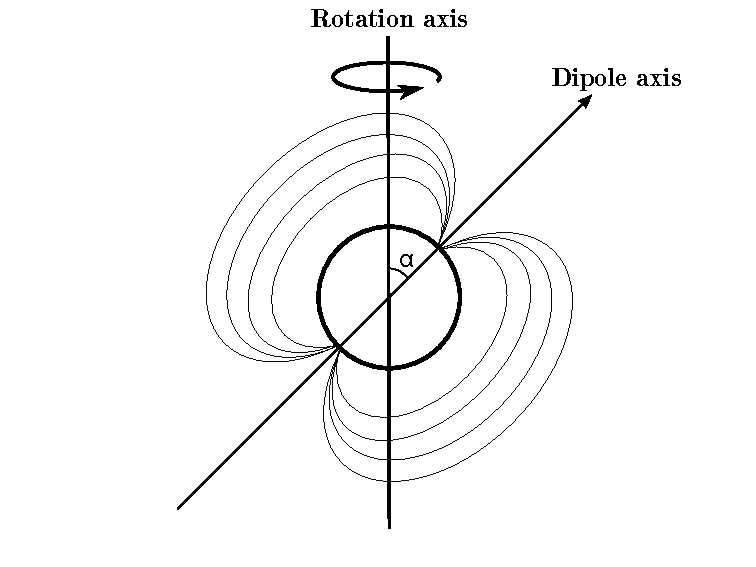
\includegraphics[width=.5\textwidth]{DipoleModelSimple}
    \caption{An illustration of the dipole spin-down model. The dipole and some 
    of the closed field lines are fixed at an angle $\alpha$ to the rotation 
    axis. As the body rotates, radiation is emitted along both ends of the dipole
    axis producing a torque on the body.}
    \label{fig: DipoleSpindownSimple}
\end{figure}

From \S 67 of \citet{Landau2013classical}, the total radiation from a dipole
rotated at angular frequency $\Omega$ can be shown to be given by
\begin{align}
\Upsilon = \frac{2}{3}\frac{\Omega^{4}}{c^{3}} d_{0}^{2},
\end{align}
where $d_0$ is the projection of the dipole moment on the plane perpendicular
to the axis of rotation \citep{Pacini1967}. We note that we could alternatively
parameterise with the pulse period $P=\frac{2\pi}{\Omega}$.
Following the arguments in \S 10.5 of \citet{Shapiro83}, the
magnitude of the magnetic dipole moment for a star with radius $R$ and surface magnetic
field strength $B_0$ is $B_{0}R^{3}/2$. Including the projection onto the
plane perpendicular to the rotation axis, the total radiation is then
\begin{align}
\Upsilon = \frac{1}{6}\frac{\Omega^{4}}{c^{3}} B_0^2 R^{6} \sin^{2}\alpha.
\end{align}

The rotational energy of a body spinning at $\Omega$ with a moment of inertia
$I_{0}$ is given by
\begin{equation}
    E = \frac{1}{2}I_{0}\Omega^{2}.
\end{equation}
Differentiating this expression with respect to time gives the loss of rotational
energy, $\dot{E}=I_0 \Omega\dot{\Omega}$ where $\dot{\Omega}$ is the angular
\emph{spin-down rate} which can be related to the changing pulse period by
$\dot{P}=-2\pi\frac{\dot{\Omega}}{\Omega^{2}}$.
Assuming that all the energy is lost
to the rotation of the dipole, hence the name rotation powered pulsars, we can
equate $\dot{E} = -\Upsilon$. We then rearrange
to give a power-law relation between the spin-down rate and the spin-frequency:
\begin{align}
\dot{\Omega} = -\frac{B_0^{2} R^{6} \sin^{2}\alpha}{6 c^{3} I_0} \Omega^{3}.
\label{eqn: n3 braking}
\end{align}

This power-law dependence is a model specific version of a more general
phenomenological power-law braking model
\begin{equation}
    \dot{\Omega} = -k \Omega^{n}.
    \label{eqn: power law spin-down}
\end{equation}
Generalising in this way suggests a powerful method to determine the type of
braking for a given pulsar. Specifically, differentiating Eqn.~\eqref{eqn: power law spin-down}
and rearranging it can be shown that
\begin{equation}
    n = \frac{\ddot{\Omega}\Omega}{\dot{\Omega}^{2}}.
    \label{eqn: measured braking index}
\end{equation}
Therefore, if $\ddot{\Omega}$ can be measured, then $n$ can be determined, and
hence used to infer the type of braking. For example, measuring $n=3$ would
indicate the pulsar braking is dominated by losses due to the magnetic dipole,
in contrast, it can be shown that gravitational wave braking would produce
$n=5$ \citep[][pg.284]{Shapiro83}. Unfortunately, in reality, pulsars do not constrain this
value. Work by \citet{Biryukov2012} found (see Figure~\ref{fig: biryukov}) that
younger pulsars tend to have braking indices of the correct order of
magnitude. However, beyond~$\tau_{ch}\approx10^{5}$~years
the absolute value of the braking index rapidly grows,
reaching values as large as $10^{6}$ for the oldest pulsar. In addition, an
almost equal number of pulsars have positive and negative values of the braking
index.
\begin{figure}[htb]
\centering
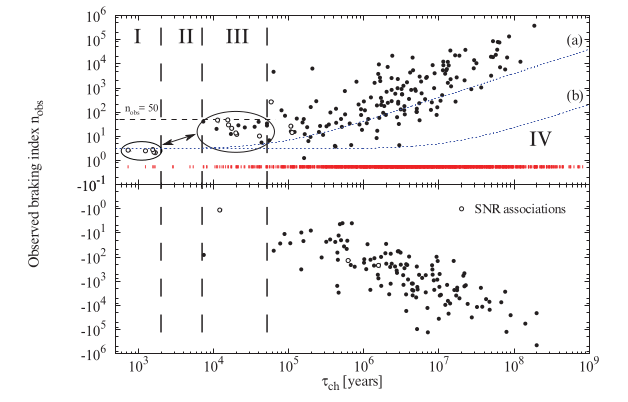
\includegraphics[width=0.8\textwidth]{Biryukov_2012_Figure_7}
\caption{The inferred observed braking index $n_{\textrm{obs}}$ against the
characteristic age $\tau_{\textrm{ch}}=\tauAge$ values for 1337 ordinary
rotation powered pulsar, figure reproduced from \citet{Biryukov2012}.}
\label{fig: biryukov}
\end{figure}

To infer the age of the pulsar, Eqn.~\eqref{eqn: power law spin-down} can
be integrated between the initial values ($t=0, \Omega=\Omega_{i}$) and the
observed value ($\Omega_{\mathrm{o}}$) to give
\begin{equation}
    t = \frac{1}{(1-n)} \frac{\Omega_{\mathrm{o}}}{\dot\Omega_{\mathrm{o}}} 
        \left(1 - \frac{\Omega_{\mathrm{o}}^{n-1}}{\Omega_{i}^{n-1}}\right).
\label{eqn: characteristic age}
\end{equation}
Typically, we make the assumption that all
pulsars, regardless of their measured braking index, are dominated by EM braking
such that $n=3$. Then additionally assuming that $\Omega_{i} \gg
\Omega_{\mathrm{o}}$ we can approximate to a characteristic age
\begin{equation}
    \tauAge = -\frac{\Omega_{\mathrm{o}}}{2\dot\Omega_{\mathrm{o}}}
         = \frac{P}{2\Pdot}.
\label{eqn: tauAge definition}
\end{equation}

To infer the approximate surface magnetic field strength, we first note that
in the EM dipole braking model:
\begin{align}
k = \frac{B_0^{2} R^{6} \sin^{2}\alpha}{6c^{3}I_0}.
\end{align}
Then rearranging Eqn.~\eqref{eqn: n3 braking} we can estimate the surface
magnetic field strength at the poles by
\begin{equation}
    B_{0} = \left(\frac{6 c^{3} I_{0}}{R^{6} \sin^{2}\alpha}\right)^{\frac{1}{2}} 
            \left(\frac{-\dot{\Omega}}{\Omega^{3}}\right)^{\frac{1}{2}}
          = \frac{1}{2\pi}\left(\frac{6 c^{3} I_{0}}{R^{6} \sin^{2}\alpha}\right)^{\frac{1}{2}}
           \sqrt{P \Pdot}
\label{eqn: surface magnetic field}
\end{equation}
In general we do not know the inclination angle $\alpha$, but we can evaluate a
minimum magnetic field strength by setting $\alpha=\pi/2$. In CGS units, for a
canonical pulsar with $R=10^{6}$~cm, $I_{0}=10^{45}$~g~cm$^{2}$, we can
approximate the magnetic field strength as $B_{0} = 6.4 \times 10^{19} \sqrt{P
\Pdot}$~Gauss. It is conventional, however, to quote the magnetic field at the equator
$B_\mathrm{s}$ which differs by a factor of 2 (see \citet{Lyne2012book} pg. 71)
such that
\begin{equation}
    B_{\mathrm{s}} = 3.2 \times 10^{19} \sqrt{P \Pdot}\textrm{ Gauss}.
\label{eqn: surface magnetic field canonical}
\end{equation}

In this section, we have introduced some of the simple results that can be
obtained by modelling the time evolution of pulsars with a power law. Many
advancements can be made on this model, such the existence of a magnetosphere
predicted by \citet{Goldreich1969}, but in practice this model is consistent
with most pulsar observations and provides a useful way to categorise them via
their spin-down age and magnetic field. We will
frequently refer back to this model as it is a useful platform from which
to begin understanding neutron stars.

